\chapter{Configuración pend para accesar directamente a los nodos de login}
Pen es una aplicación que permite el balanceo de cargas dinámicamente para páginas web, evitando la sobrecarga de los servidores cuando la demanda es alta \cite{pendhttp}. Esta utilidad se puede implementar además para otros servicios como SSH, caso para el cual se instalará y configurará esta aplicación.
%%%%%%%%%%%%%%%%%%%%%%%%%%%%%%%%%%%%%%%%%%%%%%%%%%%%%%%%%%%%%%%%%%%
Iniciamos sesión en el meta nodo, el cual se encargará de realizar esta distribución de cargas de inicio de sesión hacia los nodos de Login. Para instalar pen, hacemos lo siguiente:
%%%%%%%%%%%%%%%%%%%%%%%%%%%%%%%%%%%%%%%%%%%%%%%%%%%%%%%%%%%%%%%%%%%
\begin{lstlisting} 
yum install pen
\end{lstlisting}
%%%%%%%%%%%%%%%%%%%%%%%%%%%%%%%%%%%%%%%%%%%%%%%%%%%%%%%%%%%%%%%%%%%
Nos dirigimos a editar el archivo de configuración /etc/pen.conf y procuramos realizar los siguientes ajustes
%%%%%%%%%%%%%%%%%%%%%%%%%%%%%%%%%%%%%%%%%%%%%%%%%%%%%%%%%%%%%%%%%%%
\begin{lstlisting} 
# log file
LOGFILE=/var/log/pen.log

# statics report file
WEBFILE=/var/www/pen/webstats.html

# max connections
MAX_CONNECTIONS=256

# send X-Forwarded-For header
XFORWARDEDFOR=true

# Round-Robin mode
ROUNDROBIN=true

# listening port
PORT=80 # Temporal mientras habilitan el puerto en el CETIC

# number of backends
BACKEND=2

# define backend servers
#SERVER1=10.0.0.159:22 #laptop

SERVER1=10.0.0.10:22 # IP de Login-0
SERVER2=10.0.0.11:22 # IP de Login-1
SERVER2=10.0.0.12:22 # IP de Login-2
SERVER2=10.0.0.13:22 # IP de Login-3
\end{lstlisting}
%%%%%%%%%%%%%%%%%%%%%%%%%%%%%%%%%%%%%%%%%%%%%%%%%%%%%%%%%%%%%%%%%%%
Dado el ajuste temporal del puerto, es necesario detener el servicio web para realizar pruebas, pero una vez habilitado el puerto deseado, simplemente se cambia la configuración y se vuelve a habilitar el servicio. Mientras tanto hacemos lo siguiente:
%%%%%%%%%%%%%%%%%%%%%%%%%%%%%%%%%%%%%%%%%%%%%%%%%%%%%%%%%%%%%%%%%%%
\begin{lstlisting} 
systemctl stop httpd.service
systemctl enable pend.service
systemctl start pend.service
\end{lstlisting}
%%%%%%%%%%%%%%%%%%%%%%%%%%%%%%%%%%%%%%%%%%%%%%%%%%%%%%%%%%%%%%%%%%%
Finalmente se prueba el servicio realizando ssh desde el puerto 80 al clúster para verificar que se esté redirigiendo correctamente a los nodos de Login. En la figura \ref{fig:pen:00} se muestra una prueba de acceso satisfactorio con el demonio pen corriendo.
%%%%%%%%%%%%%%%%%%%%%%%%%%%%%%%%%%%%%%%%%%%%%%%%%%%%%%%%%%%%%%%%%%%
\begin{figure}[H]
    \centering
    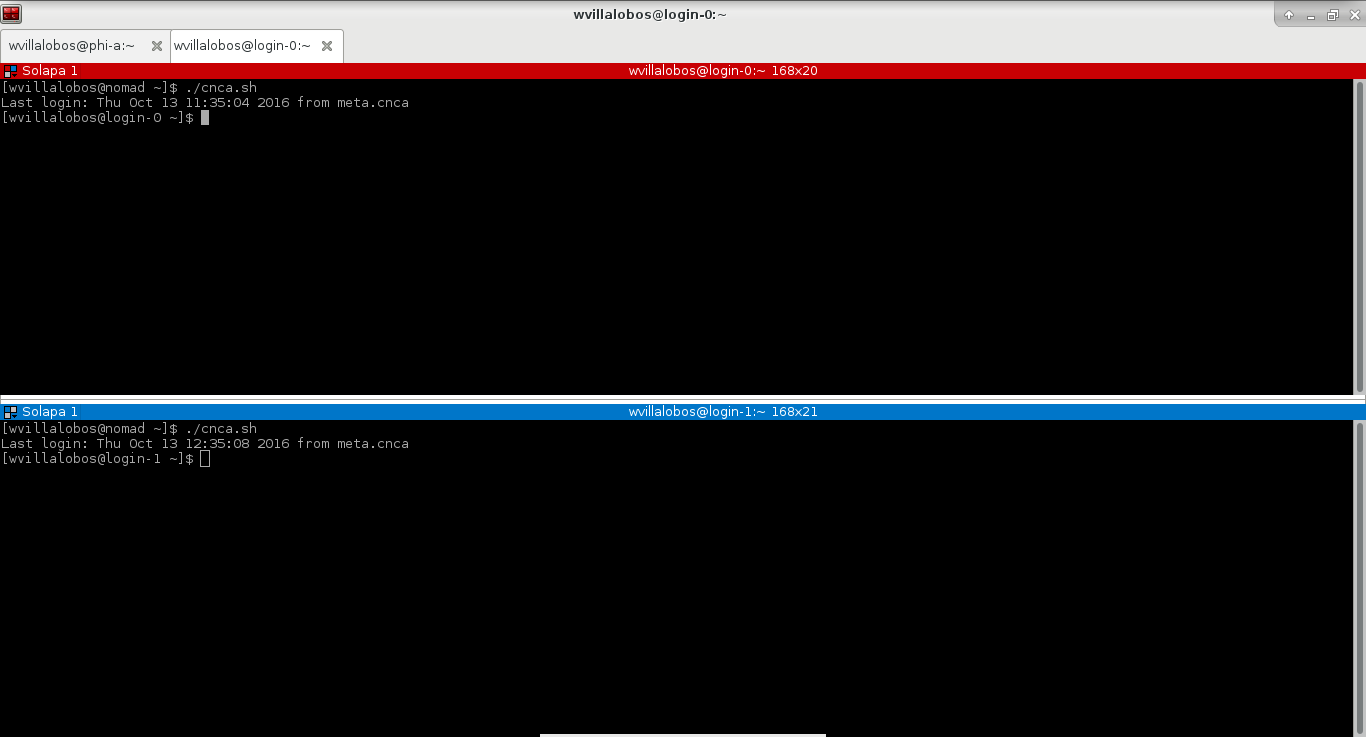
\includegraphics[width=0.5\textwidth]{pend00.png}
    \caption{Prueba de acceso distribuido con PEN.}
    \label{fig:pen:00}
\end{figure}
%%%%%%%%%%%%%%%%%%%%%%%%%%%%%%%%%%%%%%%%%%%%%%%%%%%%%%%%%%%%%%%%%%%
\begin{lstlisting} 
ssh -p80 usuario@cluster.cenat.ac.cr
\end{lstlisting}
%%%%%%%%%%%%%%%%%%%%%%%%%%%%%%%%%%%%%%%%%%%%%%%%%%%%%%%%%%%%%%%%%%%
En caso que dé error, es posible que sea necesario borrar primero el archivo /home/user/.ssh/known\_hosts para corregirlo.
%%%%%%%%%%%%%%%%%%%%%%%%%%%%%%%%%%%%%%%%%%%%%%%%%%%%%%%%%%%%%%%%%%%
\begin{lstlisting} 
@@@@@@@@@@@@@@@@@@@@@@@@@@@@@@@@@@@@@@@@@@@@@@@@@@@@@@@@@@@
@    WARNING: REMOTE HOST IDENTIFICATION HAS CHANGED!     @
@@@@@@@@@@@@@@@@@@@@@@@@@@@@@@@@@@@@@@@@@@@@@@@@@@@@@@@@@@@
IT IS POSSIBLE THAT SOMEONE IS DOING SOMETHING NASTY!
Someone could be eavesdropping on you right now (man-in-the-middle attack)!
It is also possible that the RSA host key has just been changed.
The fingerprint for the RSA key sent by the remote host is
62:ce:d6:b2:8b:5e:10:8e:9d:42:49:9a:f9:85:94:f5.
Please contact your system administrator.
Add correct host key in /home/wvillalobos/.ssh/known_hosts to get rid of this message.
Offending key in /home/wvillalobos/.ssh/known_hosts:1
RSA host key for login-0 has changed and you have requested strict checking.
Host key verification failed.

rm .ssh/known_hosts 
\end{lstlisting}

Lo anterior es un arreglo temporal el cual seguirá dando conflicto conforme se agreguen nuevos nodos login al sistema. Lo ideal es homologar las llaves privadas en los nodos login nuevos para asegurar que no exista conflictos cuando se inicie sesión por ssh. Para esto, respaldamos los archivos de la carpeta /etc/ssh en /etc/ssh/orig y copiamos los archivos de uno de los nodos login ya instalados.

\begin{lstlisting}
cd /etc/ssh
mkdir orig
cp ./* orig/
scp login-0:/etc/ssh/ .
chmod 600 *.key
\end{lstlisting}

Lo anterior nos asegura que los nodos login tengan la misma llave privada, además de garantizar que tengan los permisos adecuados para evitar problemas con el proceso de cifrado y seguridad de los equipos. Además elimina permanentemente el error de autentificación mostrado.

%%%%%%%%%%%%%%%%%%%%%%%%%%%%%%%%%%%%%%%%%%%%%%%%%%%%%%%%%%%%%%%%%%%
\section{Homologación del archivo known\_hosts, skel y generación de llaves en inicio de sesión por primera vez}
La configuración del servicio pend implica que ahora el servicio ssh del cliente 
piense que hay un ataque, tal y como se indicó previamente. En el meta nodo, en el directorio /etc/skel/.ssh se ha copiado una versión del known\_hosts actualizada para facilitar a nivel de clúster la comunicación a través de ssh para los nuevos usuarios. Además, se creó el script khosts.sh para reemplazar todos los known\_hosts en cada uno de los usuarios ya existentes \cite{loopbash}:
%%%%%%%%%%%%%%%%%%%%%%%%%%%%%%%%%%%%%%%%%%%%%%%%%%%%%%%%%%%%%%%%%%%
\lstinputlisting{khosts.sh}
Si observamos con atención el script, observamos que se requiere copiar un script llamado generarLlave.sh. Este script lo que permite es crear las llaves ssh en el primer  inicio de sesión, de manera que facilita el inicio de sesión en cada uno de los nodos del clúster Kabré. Dicho script se copia a /etc/profile.d y contiene lo siguiente:

\lstinputlisting{generarLlave.sh}
%%%%%%%%%%%%%%%%%%%%%%%%%%%%%%%%%%%%%%%%%%%%%%%%%%%%%%%%%%%%%%%%%%%
Para ejecutar este script, simplemente hacemos lo siguiente como root:
%%%%%%%%%%%%%%%%%%%%%%%%%%%%%%%%%%%%%%%%%%%%%%%%%%%%%%%%%%%%%%%%%%%
\begin{lstlisting} 
chmod +x khosts.sh # En caso de que no sea ejecutable
./khosts.sh
\end{lstlisting}
%%%%%%%%%%%%%%%%%%%%%%%%%%%%%%%%%%%%%%%%%%%%%%%%%%%%%%%%%%%%%%%%%%%
\clearpage